\section{Module 9. Segmentation}

Image segemntation is very important part of medical processing. Segmentation is the process clustering an image pixels into region of interest with similar properties. Many image segmentation alghoritm is used in medical applications to segment body organs and tissues. Some of the application  consist of surgical planning, tumor detection and segmentation, brain development study, heart segme tation, etc. For example, MRI segmentation is commonly used for measuring and visualizing different brain structures, for delineating lesions, for analysing brain development, and for image-guided interventions and surgical planning.  

This process can prove useful in clustering the specific brain regions in MRI image. Partition the image into different region colours can vizualize grey matter, white metter and cerebrospinal fluid in brain image. 

In this documenation, we focuse only on brain segmentation and describe an alghoritm, which is used in application.

\textbf{\textit{Image segmentation}}
The real purpose of image segmentation is to subdivided an image into nonoverlapping, semantically meaningful and homogeneous regions with similar features, such as: colour, depth, intensity or texture. The basic part of structural brain MRI analysis  is MRI data classification into appropriate tissue types, recognition and description of specific anatomical structures.
Classification means assignment to each element in the image a tissue class. The problems of classification and segmentation are interlinked, because classification is the result of segmentation and  a classifier implicitly segments an image. In brain MRI segmentation, image pixels are typically classified into three main tissue types:  cerebrospinal fluid (CSF), gray matter (GM)  and white matter (WM)(Fig. \ref{fig:figures/m09_1}). 

\begin{figure}[H]
\centering{}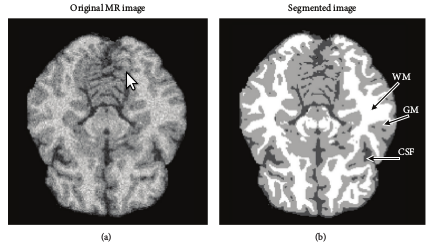
\includegraphics[width=0.7\textwidth]{figures/Module_09/m09_1} \caption{The brain MRI segmentation with a) original MRI image and b) image after segemntation with three labels: CFS, GM and WM  \label{fig:figures/m09_1}}
\end{figure}

Most of the image segmentation research has focused on 2D images. For the data, which is defined in 3D space - a series of MRI images, then typically each image “slice” is segmented individually in a “slice-by-slice” manner. In practice, 2D image segmentation methods can be extended to 3D space, but often with the cost of an increased complexity of the method and slower computational time.\\

\textbf{\textit{MRI preprocessing}}
To prepare brain MRI images for segmentation, it is necessary to perform several preprocessing steps (Fig. \ref{fig:figures/m09_2}). One of the most important features for brain MRI segmentation is the intensity of brain tissue. However, intensity-based segmentation algorithms will lead to wrong results when intensity value are corrupted by MRI artifacts. The most important preprocessing steps are:
\begin{itemize}
\item the MRI bias field correction,
\item image registration, 
\item skull stripping and nonbrain tissue removing – brain extraction
\end{itemize}

Trained medical experts can make visual MRI analysis to certain levels of intensity inhomogeneity, in contrast, the performance of intensity-based segmentation methods and automatic MRI analysis decreases greatly in the presence of the bias field (Fig. \ref{fig:figures/m09_3}).

\begin{figure}[H]
\centering{}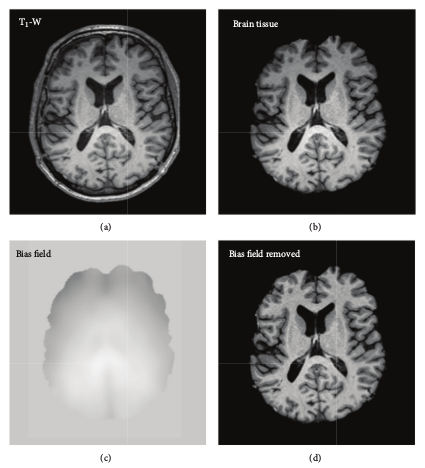
\includegraphics[width=0.7\textwidth]{figures/Module_09/m09_2}\caption{Preprocessing steps: a) the original T1 brain MRI image, b) the brain tissue image after skull stripping, c)  the bias field, d) the brain tissue image after the bias field correction \label{fig:figures/m09_2}}
\end{figure}

\begin{figure}[H]
\centering{}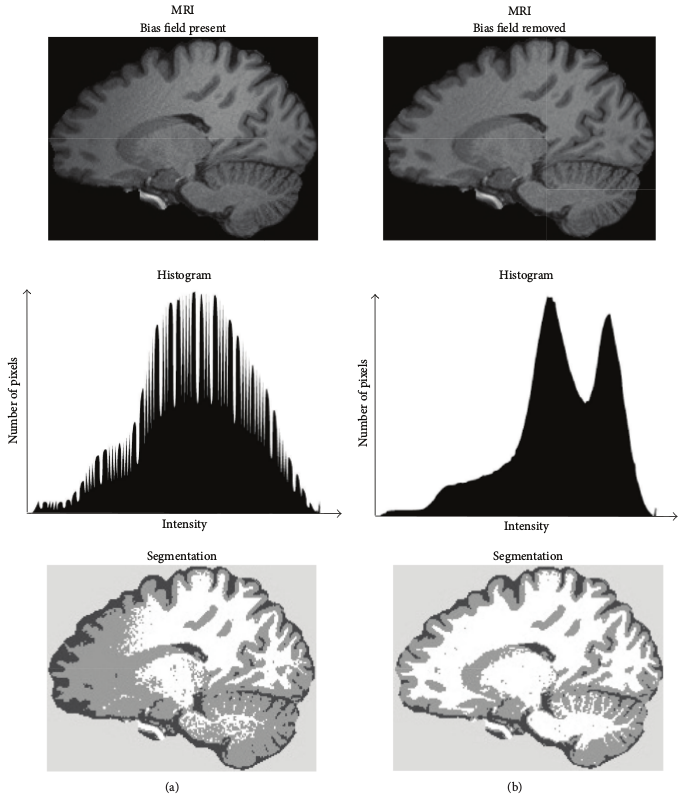
\includegraphics[width=0.7\textwidth]{./figures/Module_09/m09_3}\caption{Influence of the bias field on brain MRI segmentation  \label{fig:figures/m09_3}}
\end{figure}

The second, very important preprocessing step is to remove nonbrain tissue. Tissues such as skull, fat or neck have intensities overlapping with intensities of brain tissues. Which means, that only skull stripping is not enough to segmentation whole brain image. The result of removing nonbrain elements can be either a binary mask , which has a value of 1 for brain voxels and 0 for the rest of tissues or a new image with just brain voxels. The brain voxels comprise GM, WM, and CSF of the cerebral cortex and subcortical structures, including the brain stem and cerebellum.

\textbf{\textit{MRI segmentation methods}}
Automated analysis of MR images is challenging due to intensity inhomogeneity, variability of the intensity ranges and contrast, noise or other image-artifacts. There is no single alghoritm that can be suitable for all images. Most of the segmentation methods developed for one class of images can be easily applied/extended to another class of images. For example, the theory of graph cuts, although firstly developed for binary images, can be modified and used for MRI segmentation of the brain tissue. The segmentation methods, with application to brain MRI, may be grouped as follows:
\begin{itemize}
\item manual segmentation, 
\item intensity-based methods (including thresholding, region growing, classification, and clustering),
\item atlas-based methods,
\item surface-based methods (including active contours and surfaces, and multiphase active contours),
\item hybrid segmentation methods.
\end{itemize}

\textbf{\textit{Segmentation method used in application}}
In application, the Gaussian Mixture Model (GMM) based on Expectation-Maximization (EM) algorithm  is used to extract specific brain tissues. This is one of clustering methods, which are unsupervised segmentation methods that partition an image into clusters of pixels/voxels with similar intensities without using training images. In fact, clustering methodes use the available image data to train themselves. Both, the segmentation and training, are done in parallel by iterating steps. 

\textit{Daussian mixture model}
Often the data we are trying to model is much more complex, then simple distributions, like Bernoulli or Gaussian.  For instance, it might be multimodal.  This means  that  there  are  several  different modes,  or  regions  of  high  probability  mass,  and regions of smaller probability mass in between. An excample can be image. In this case, it is possible to model the data in terms of a mixture of several components, where each component has a simple parametric form (such as a Gaussian).
The Gaussian mixture model is simple linear superposition of Gaussian components, aimed at providing a richer class of density models than the single Gaussian. Mixture model i probabilistic model, which can represent the presence of subpopulations within an overall population. 
The Gaussian distribution in mixture model (Fig. \ref{fig:figures/m09_4}) can be written in the form \ref{Eq: wz_1}.


The probability given in mixture of K Gaussians is 

\begin{figure}[h]
\centering{}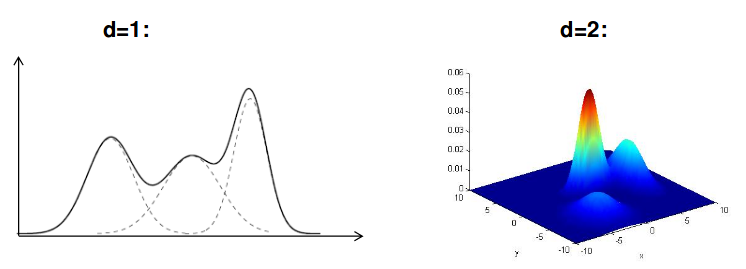
\includegraphics[width=0.7\textwidth]{figures/Module_09/m09_4}\caption{Gaussian mixture model examples for 1 and 2 dimension  \label{fig:figures/m09_4}}
\end{figure}

Gaussaian mixture model can be attached to set of data  with an unknown distribution, by estimate the parameters (theta) of GMM model that fits the data. The solution is to maximize the likelihood p(X|theta) of the data with regard to the model parameters. 

\textit{\textbf{List of References}}\\
\cite{09a1}